
%%%%%%%%%%%%%%%%%%%%%%%%%%%%%%%%%%%%%%%%%%%%%%%%%%%%%%%%%%%%%%%%%%%%%%%%
% FOLLOWUP TEXT IS OLDER AND MAY NEED MERGING OR DISCARDING
%%%%%%%%%%%%%%%%%%%%%%%%%%%%%%%%%%%%%%%%%%%%%%%%%%%%%%%%%%%%%%%%%%%%%%%%

\newpage
\appendix

\section{Exhaustive Results}

\begin{figure*}[t]
\noindent\begin{tabular}{C{.5\linewidth}C{.5\linewidth}}
For fixed values of the platform bandwidth & For fixed values of the platform MTBF \\
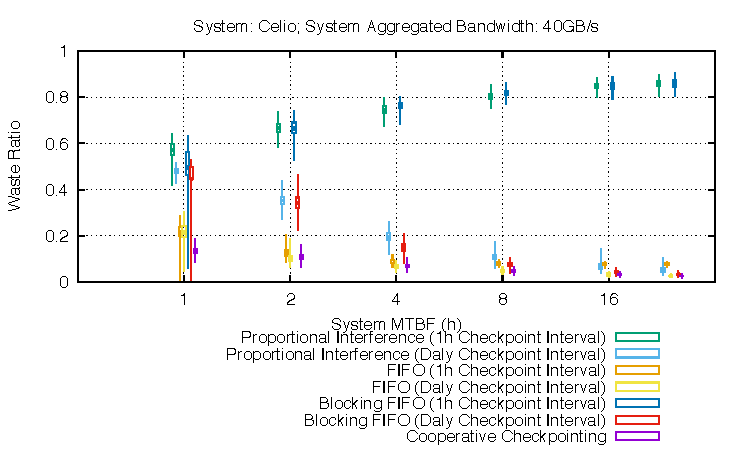
\includegraphics[width=\linewidth]{sim/figures/synthetic-040gbs-waste-celio.pdf} & 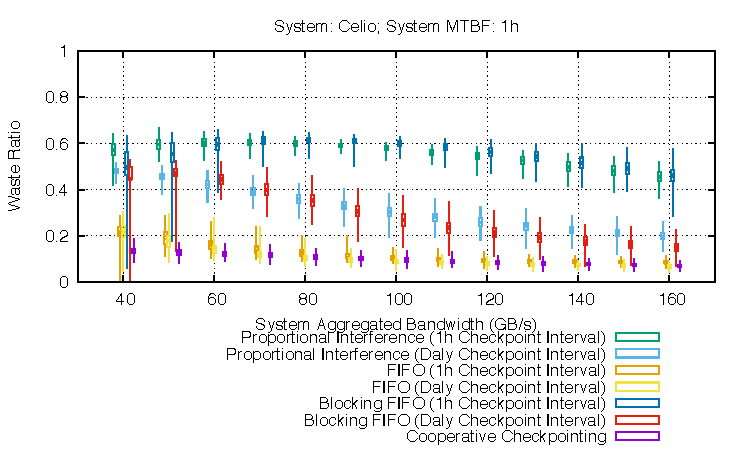
\includegraphics[width=\linewidth]{sim/figures/synthetic-01hMTBF-waste-celio.pdf} \\
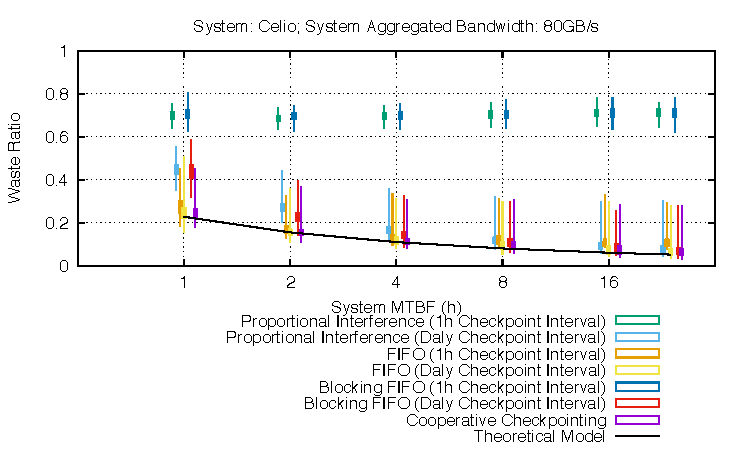
\includegraphics[width=\linewidth]{sim/figures/synthetic-080gbs-waste-celio.pdf} & 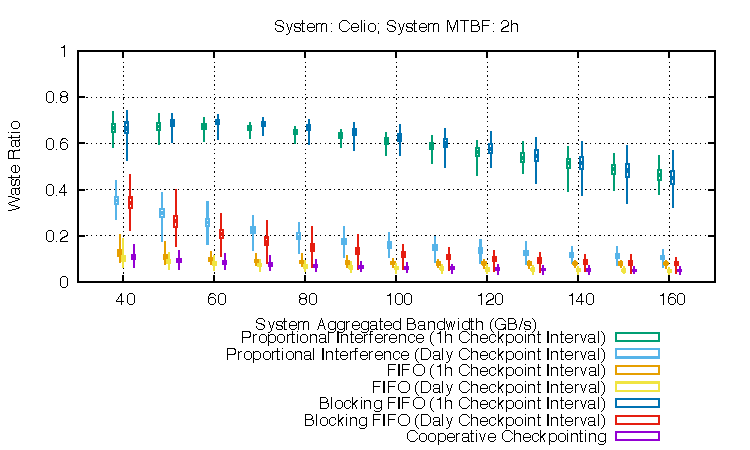
\includegraphics[width=\linewidth]{sim/figures/synthetic-02hMTBF-waste-celio.pdf} \\
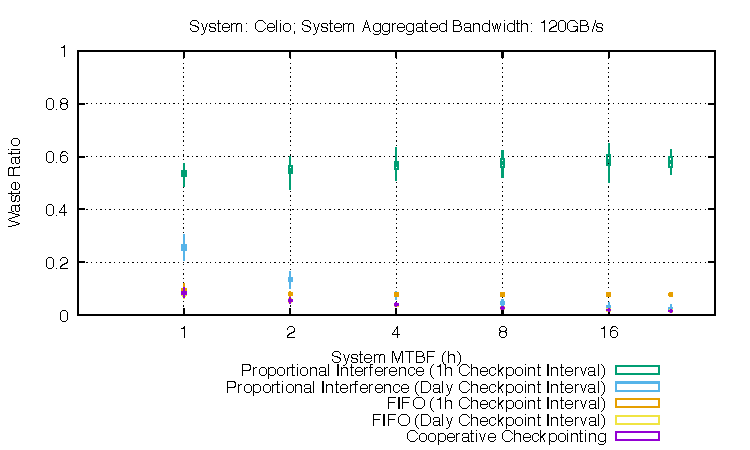
\includegraphics[width=\linewidth]{sim/figures/synthetic-120gbs-waste-celio.pdf} & 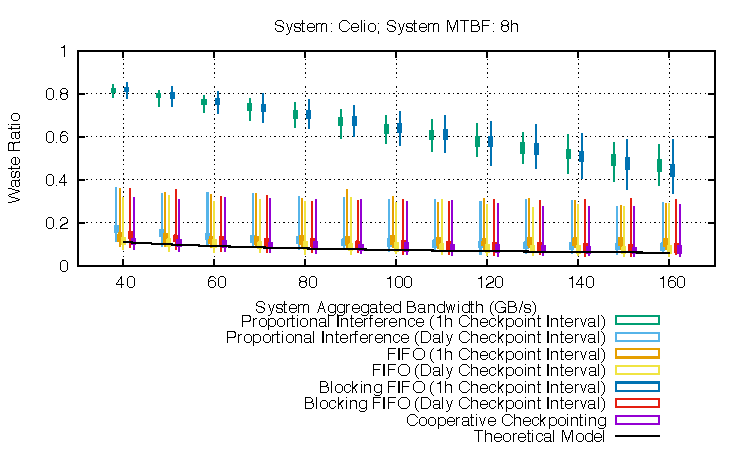
\includegraphics[width=\linewidth]{sim/figures/synthetic-08hMTBF-waste-celio.pdf} \\
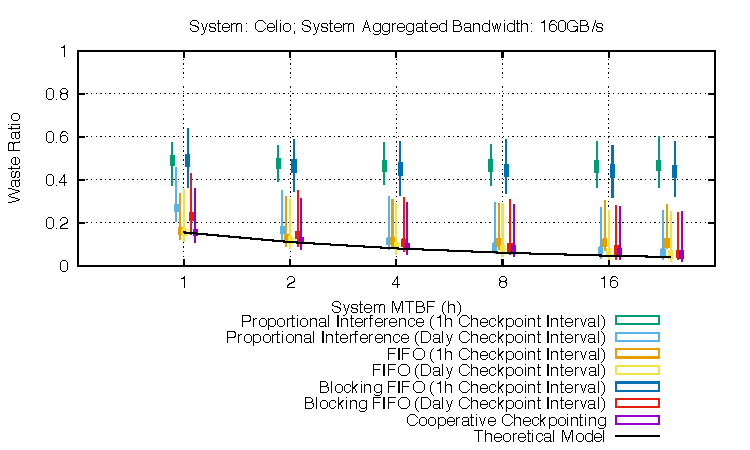
\includegraphics[width=\linewidth]{sim/figures/synthetic-160gbs-waste-celio.pdf} & 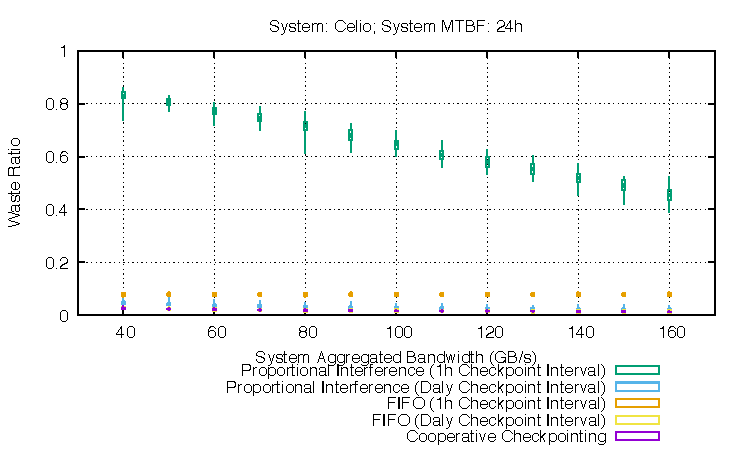
\includegraphics[width=\linewidth]{sim/figures/synthetic-24hMTBF-waste-celio.pdf} \\
\end{tabular}
\caption{Celio, Waste}
\end{figure*}

\clearpage

\begin{figure*}[t]
\noindent\begin{tabular}{C{.02\linewidth}C{.49\linewidth}C{.49\linewidth}}
     ~    &  Checkpoint Period: 1H & Checkpoint Period: Daly \\
\rotatebox[origin=c]{90}{Overall Waste} & 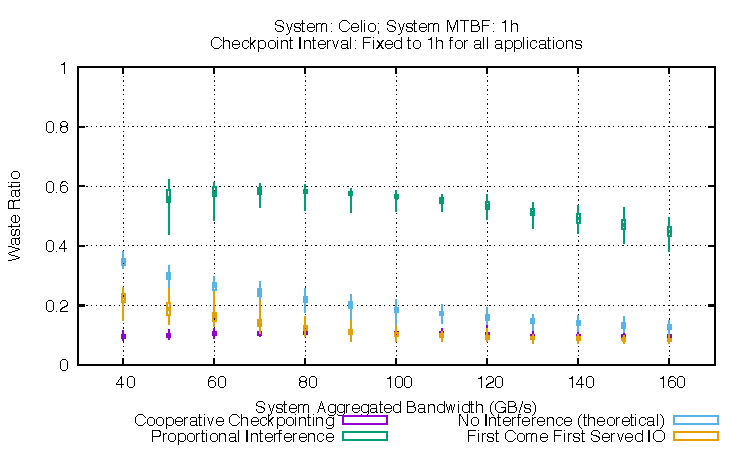
\includegraphics[width=\linewidth]{sim/figures/1hMTBF-1hckpt-waste-celio.pdf} & 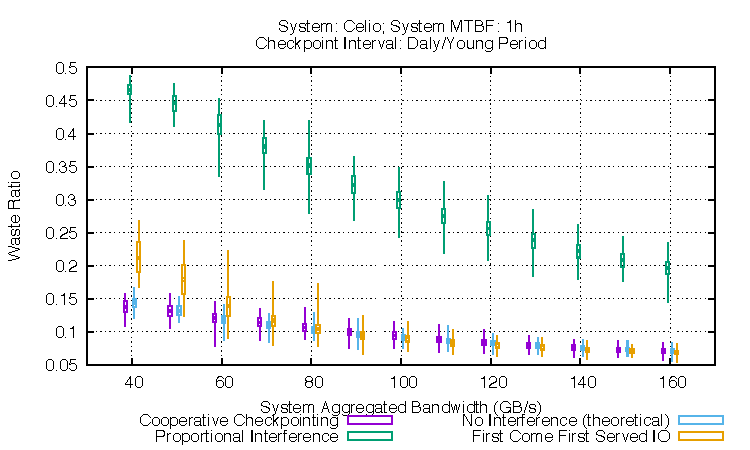
\includegraphics[width=\linewidth]{sim/figures/1hMTBF-dalyckpt-waste-celio.pdf} \\
\rotatebox[origin=c]{90}{Checkpointing} & 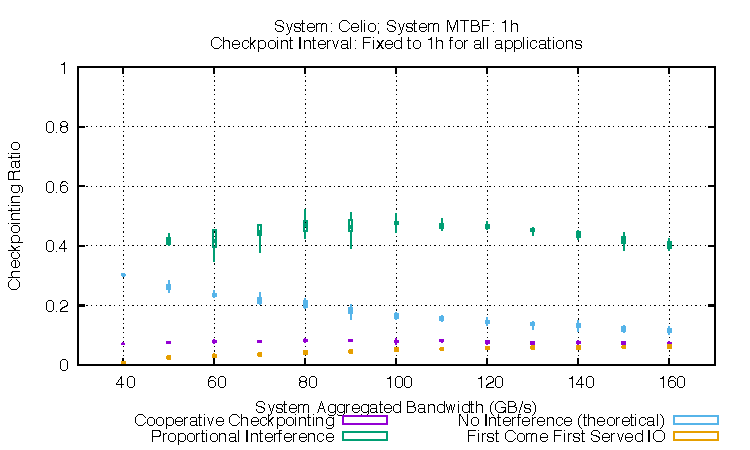
\includegraphics[width=\linewidth]{sim/figures/1hMTBF-1hckpt-ckpt-celio.pdf} & 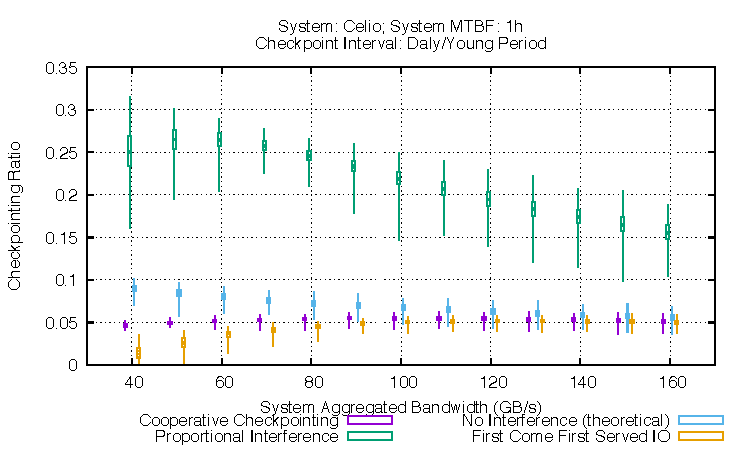
\includegraphics[width=\linewidth]{sim/figures/1hMTBF-dalyckpt-ckpt-celio.pdf} \\
\rotatebox[origin=c]{90}{Usefull Work} & 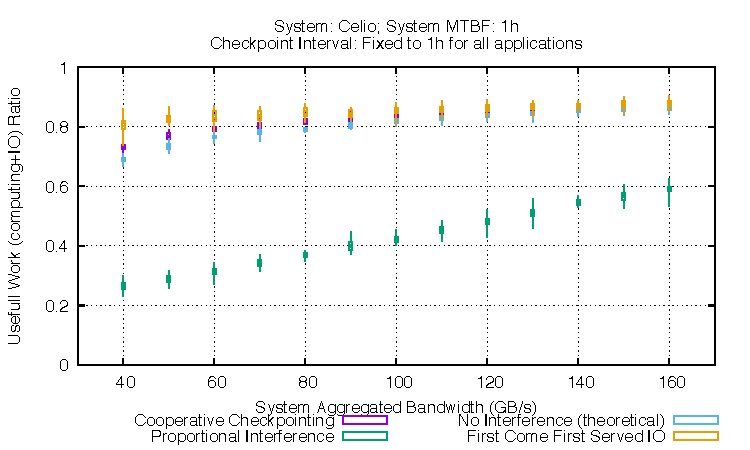
\includegraphics[width=\linewidth]{sim/figures/1hMTBF-1hckpt-work-celio.pdf} & 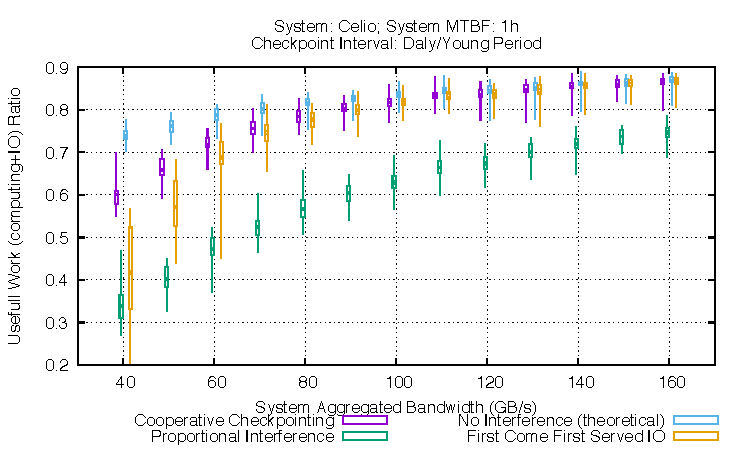
\includegraphics[width=\linewidth]{sim/figures/1hMTBF-dalyckpt-work-celio.pdf} \\
\rotatebox[origin=c]{90}{Usefull I/O} & 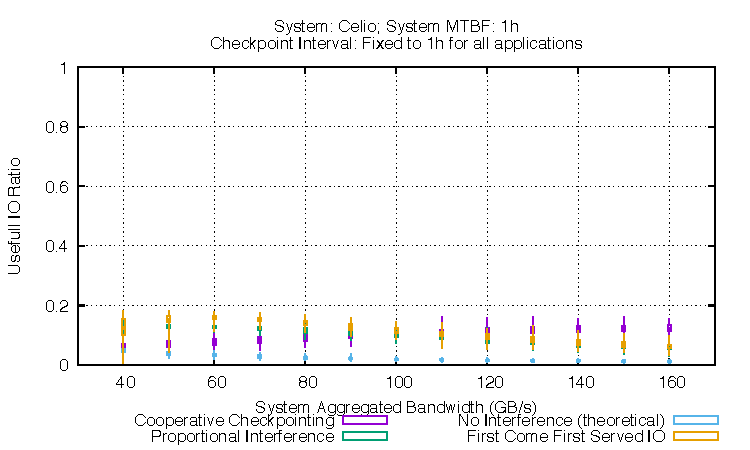
\includegraphics[width=\linewidth]{sim/figures/1hMTBF-1hckpt-io-celio.pdf} & 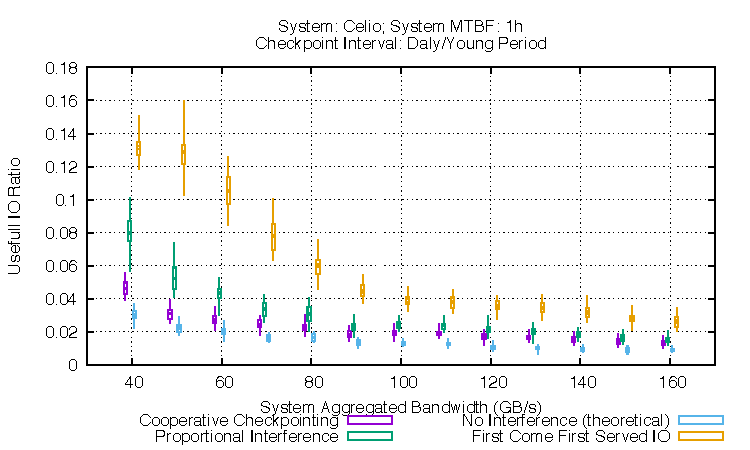
\includegraphics[width=\linewidth]{sim/figures/1hMTBF-dalyckpt-io-celio.pdf}
\end{tabular}
\caption{Celio, Fixed MTBF: 1H}
\end{figure*}

\clearpage

\begin{figure*}[t]
\noindent\begin{tabular}{C{.02\linewidth}C{.49\linewidth}C{.49\linewidth}}
     ~    &  Checkpoint Period: 1H & Checkpoint Period: Daly \\
\rotatebox[origin=c]{90}{Overall Waste} & 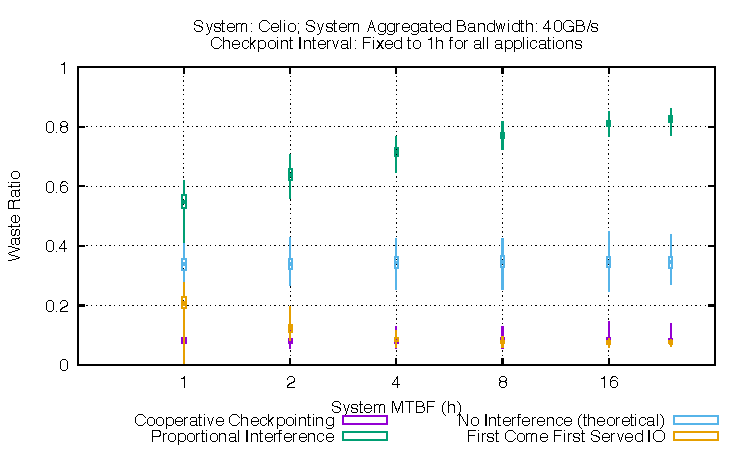
\includegraphics[width=\linewidth]{sim/figures/40gbs-1hckpt-waste-celio.pdf} & 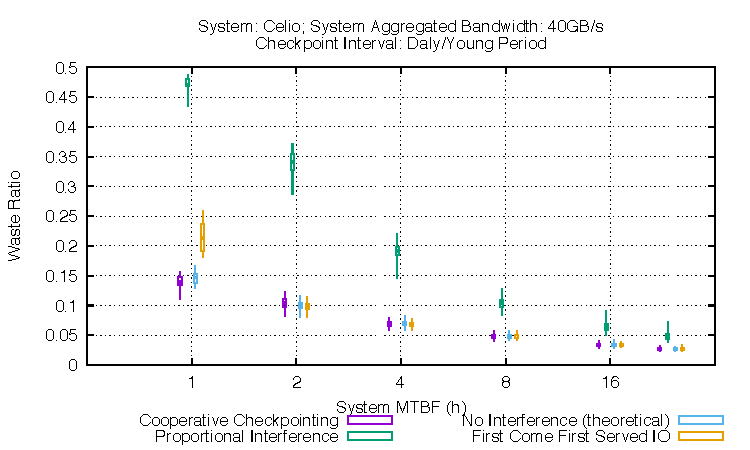
\includegraphics[width=\linewidth]{sim/figures/40gbs-dalyckpt-waste-celio.pdf} \\
\rotatebox[origin=c]{90}{Checkpointing} & 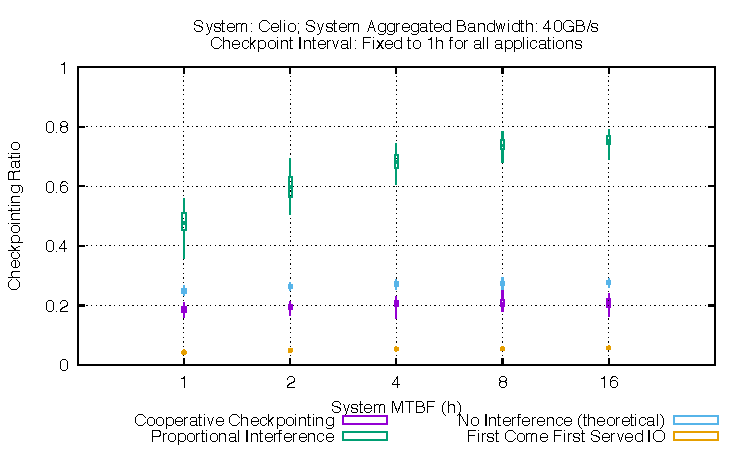
\includegraphics[width=\linewidth]{sim/figures/40gbs-1hckpt-ckpt-celio.pdf} & 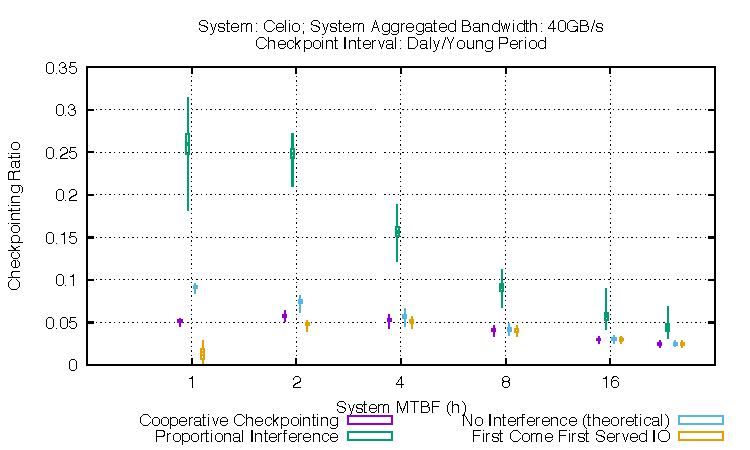
\includegraphics[width=\linewidth]{sim/figures/40gbs-dalyckpt-ckpt-celio.pdf} \\
\rotatebox[origin=c]{90}{Usefull Work} & 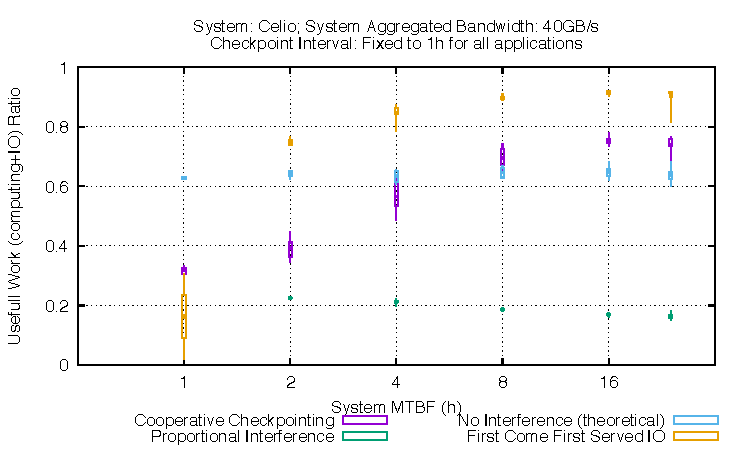
\includegraphics[width=\linewidth]{sim/figures/40gbs-1hckpt-work-celio.pdf} & 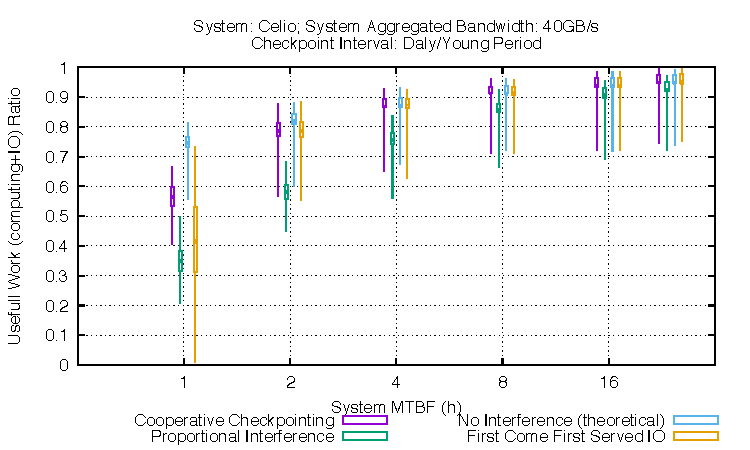
\includegraphics[width=\linewidth]{sim/figures/40gbs-dalyckpt-work-celio.pdf} \\
\rotatebox[origin=c]{90}{Usefull I/O} & 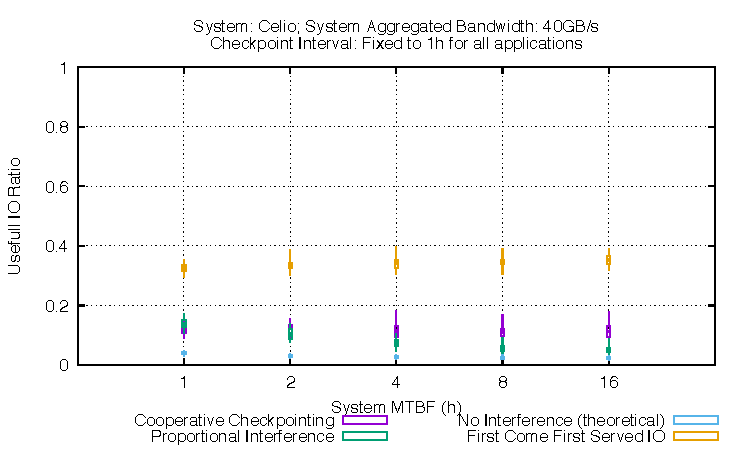
\includegraphics[width=\linewidth]{sim/figures/40gbs-1hckpt-io-celio.pdf} & 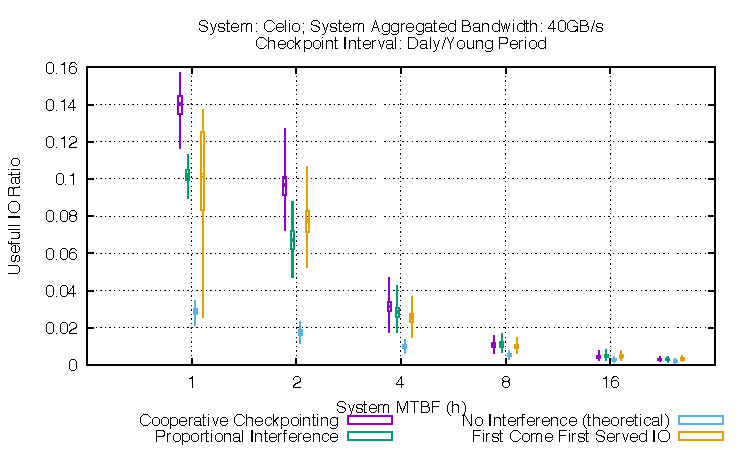
\includegraphics[width=\linewidth]{sim/figures/40gbs-dalyckpt-io-celio.pdf}
\end{tabular}
\caption{Celio, Fixed Bandwidth: 40GB/s}
\end{figure*}

\clearpage


\section{Older text}



\subsection{Checkpointing and I/O}

For a single application, the optimal checkpointing period is given by the Young/Daly
formula~\cite{young74,daly04}. This period minimizes the platform waste, defined as
the fraction of the
execution time that does not contribute to the progress of the application (the
time \emph{wasted}).  There are two sources of waste, the time spent taking checkpoints
(which calls for longer checkpoint periods),
and the time needed to recover and re-execute after each failure
(which calls for shorter checkpoint periods),
The Young/Daly
period achieves the optimal trade-off between both sources to minimize the
total waste.
However, this optimal period may put too much pressure
on the I/O system. It is possible to use a longer, sub-optimal, period that would incur
less pressure and still lead to a reasonable waste. S. Arunagiri et al.~\cite{Arunagiri2009} have studied such trade-offs and they have shown, both analytically and instantiating the model with four real-life platforms,
that a great decrease in I/O requirement can be achieved  at the price of a small increase of the waste.

\subsection{I/O interference}


\section{Execution Model}
\label{sec.model}


\section{Optimal Checkpointing Period under I/O constraint}
\label{sec.optimal}

The waste of an application is the ratio of time that the application spends doing
resilience operations by the time that it does useful work. The time
spent doing resilience operations include the time spend during each period to checkpoint, and in case of failure, the time to rollback to the previous checkpoint, and the time to recompute lost work. We assume
that the rollback time is equivalent to the checkpoint time, and we
can define the waste $\wasteapp{i}$ of an application of class
$\app{i}$ as follows (\cite{springer-monograph}):

\begin{equation}
\wasteapp{i} = \wastefct{i}{\ckpt{i}} = \frac{\ckpt{i}}{\period{i}} +
\frac{\nbnodes{i}}{\mtbfplat}(\frac{\period{i}}{2} + \ckpt{i})
\label{eq.wasteAi}
\end{equation}

Let $\wasteplat$ be the waste of the platform. We define this as the
weighted arithmetic mean of the $\wasteapp{i}$ for all applications
(where each application is weighted by the number of computing nodes
it uses):

\begin{equation}
\wasteplat = \sum_i \frac{\nbapp{i} \nbnodes{i}}{\nbnodesplat} \wasteapp{i}
\label{eq.waste}
\end{equation}

In the absence of I/O constraints, the checkpointing period can be minimized
for each application independently. Indeed, the optimal period for an application
of class $\app{i}$ is obtained by minimizing $\wasteapp{i}$ in Equation~\eqref{eq.wasteAi}.
Differentiating and solving
$$\frac{\delta \wasteapp{i}}{\delta \period{i}} = - \frac{\ckpt{i}}{\period{i}^{2}} + \frac{\nbnodes{i}}{2 \mtbfplat} = 0$$
we readily derive that
\begin{equation}
\period{i} = \sqrt{2 \frac{\mtbfplat}{\nbnodes{i}} \ckpt{i}} = \sqrt{2 \mu_{i} \ckpt{i}}
\label{eq.daly}
\end{equation}
where $\mu_{i}$ is the MTBF of  class $\app{i}$ applications, which is the Young/Daly formula~\cite{young74,daly04}.
\todo[inline]{So they were right! We might want to define what $\period{i}$
  stands for before the reader reaches this point and can figure it by
  itself}

However, I/O constraints impose the use of sub-optimal periods. If each application
of  class $\app{i}$ checkpoints in time $\ckpt{i}$ during its period $\period{i}$ (hence without any contention), it uses the I/O device during a fraction $\frac{\ckpt{i}}{\period{i}}$ of the time.
The total usage fraction of the  I/O device is $\sum_{i} \frac{\nbapp{i} \ckpt{i}}{\period{i}}$
and cannot exceed $1$. Therefore, we have to solve the following optimization problem: find
the set of values $\period{i}$ that minimize $\wasteplat$ in Equation~\eqref{eq.waste} subject to the I/O constraint:

\begin{equation}
\sum_{i} \frac{\nbapp{i} \ckpt{i}}{\period{i}} \leq 1
\label{eq.IOconstraint}
\end{equation}

Note that Equation~\eqref{eq.IOconstraint} is a necessary condition, but is may not be sufficient:
even though the total I/O bandwidth is not exceeded, meaning there is enough capacity to take all the checkpoints at the given periods, we still need to orchestrate these checkpoints so that there is no contention. We come back to this point below.

The optimization problem writes: minimize $\wasteplat = \sum_i \frac{\nbapp{i} \nbnodes{i}}{\nbnodesplat}  \left( \frac{\ckpt{i}}{\period{i}} +
\frac{\nbnodes{i}}{\mtbfplat}(\frac{\period{i}}{2} + \ckpt{i}) \right)$
subject to $\ioconstraint = \sum_{i} \frac{\nbapp{i} \ckpt{i}}{\period{i}} \leq 1$.
Using the Karush-Kuhn-Tucker condition, we know that there exists a nonnegative constant
$\lambda$
such that
$$- \frac{\delta \wasteplat}{\delta \period{i}} = \lambda \frac{\delta\ioconstraint }{\delta \period{i}}$$
for all $i$. We derive that
$$\frac{\nbapp{i} \nbnodes{i} \ckpt{i}}{\nbnodesplat \period{i}^{2}} -    \frac{\nbapp{i} \nbnodes{i}^{2}}{2 \mtbfplat \nbnodesplat} = - \lambda \frac{\nbapp{i} \ckpt{i}}{\period{i}^{2}}
$$
for all $i$. This leads to:
 \begin{equation}
\period{i} = \sqrt{\frac{2 \mtbfplat  \nbnodesplat}{\nbnodes{i}^{2}} \left(\frac{\nbnodes{i}}{\nbnodesplat} +\lambda \right) \ckpt{i}}
  \label{eq.KKT}
\end{equation}
for all $i$. Note that when $\lambda=0$, Equation~\eqref{eq.KKT} reduces to Equation~\eqref{eq.daly}. Because of the I/O constraint in Equation~\eqref{eq.IOconstraint},
we will choose for $\lambda$ the minimum value such that Equation~\eqref{eq.IOconstraint}
  is satisfied. This will lead to periods $P_{i}$ larger than the optimal value of Equation~\eqref{eq.daly}.
  Note that there is no closed-form expression for the minimum value of $\lambda$,
  it has to be found numerically.
   Altogether, we state our main result:

   \begin{theorem}
  In the presence of I/O constraints, the optimal values of the checkpointing periods are given
  by Equation~\eqref{eq.KKT}, where $\lambda$ is the smallest nonnegative value such that
  Equation~\ref{eq.IOconstraint} holds.
\end{theorem}

\section{Optimal Cooperative Checkpointing Strategy}
\label{sec.strategy}

\subsection{With Burst Buffers}

We slightly change the machine model, and will consider that, in addition
to the global PFS, each node is provisioned with a local stage-in I/O
burst buffer. With burst buffers, $\ckpt{i}$ still represents the time it
takes to upload the checkpoint to the stable storage (the file system).
However, the availability of burst buffers permits a reduction in the
apparent time for the checkpoints as experienced by application idle
time. Note that under I/O constraints on the PFS, checkpoints may remain
in burst buffers (which is not a stable storage) until sufficient
PFS bandwidth is available.

Consider Algorithm~\ref{alg.withbb}: every $\period{i}$ time
units, each application of class $\app{i}$ takes a checkpoint and save
it onto the next free slot on the burst buffer; a global shared FIFO
queue transfers checkpoints from active slots in burst buffers onto
the parallel file system following the FIFO queue order.

\algblockdefx{Process}{EndProcess}[1]{\textbf{On Process} #1}{\textbf{End Process}}
\algnotext{EndProcess}
\algblockdefx{Every}{DoneEvery}[1]{\textbf{Every } #1}{\textbf{Done}}
\algnotext{DoneEvery}
\algblockdefx{When}{DoneWhen}[1]{\textbf{When } #1}{\textbf{Done}}
\algnotext{DoneWhen}
\algloopdefx{If}[1]{\textbf{If} #1 \textbf{then}}
\begin{algorithm}
\caption{Cooperative Checkpointing Algorithm with Burst Buffers}
\label{alg.withbb}
\begin{algorithmic}
\State \textbf{var} $transfer\_queue$, a FIFO initially empty
\Process{$p$, belonging to application $\application{i}{j}$ of class $\app{i}$}
   \State \textbf{var} $slots$ set of burst buffer files that can
   store a checkpoint
   \Every{$\period{i}$ time units}
           \State $slot  \gets $ oldest slot that is not being used for transfer
           \State Checkpoint application state into $slot$
           \If{$slot$ is marked done transferring}
                  \State Append $(p, slot)$ to $transfer\_queue$
    \DoneEvery
\EndProcess

\Process{$T$}
   \When{$transfer\_queue$ is not empty}
       \State Pop $slot$ from $transfer\_queue$
       \State Mark $slot$ as being transferred
       \State Transfer Checkpoint in $slot$ to File System
       \State Mark $slot$ as done transferring
   \DoneWhen
\EndProcess
\end{algorithmic}
\end{algorithm}

\begin{theorem}
  Algorithm~\ref{alg.withbb} ensures that all applications of class $\app{i}$
  checkpoint at most every $max(\sum_j\nbapp{j}*\ckpt{j}, \period{i})$
  time units, and requires only a burst buffer capable of storing 2
  checkpoints per process.
\end{theorem}

\begin{proof}
  \todo{This derives from $\sum_i \frac{\ckpt{i}}{\period{i}} \leq 1$,
    but should be done properly.}
\end{proof}

The theorem does provide a lower bound for the platform waste.\todo[inline]{the 2 storages holds only after the optimization, doesn't it? Or is it also a consequence of the above "proof" sketch?}
However, we have a FIFO system, and some applications may incur
a re-execution time larger than $P_{i}$. What is the worst case?
A first optimization is the following: when a checkpoint is taken
    by a given application, we check whether its previous checkpoint is
    still in the queue from the burst buffer to the file system. If yes, the new
checkpoint should \emph{replace} the old one, keeping the same position in the queue.
With this optimization, there is at most two checkpoints per application in the queue,
one being currently transferred and one waiting.
Then the worst case is to wait for the checkpoint of all the other applications.
Formally, the maximal re-execution time for application
$\application{i}{j}$ of class
$\app{i}$ is
$$\max(P_{i}, \sum_{k=1}^{\nbapps} n_{k}C_{k} - C_{i})$$

 \todo[inline]{Discussed at JLESC meeting: size of burst buffer can be
    bounded by 2 checkpoints easily, and it should be: if there are 3
    checkpoints in the burst buffer, then the first one might be being
    transferred, but this means that the 2nd is useless as we already
    reached the 3rd one. The 2nd should be discarded and its slot in
    the FIFO queue should be taken by the 3rd.}

  \todo[inline]{No clear what qualifies for burst buffers here, but
    currently the NVM bandwidth is (1) significantly lower than the
    network bandwidth, and (2) unidirectional. This might change in
    the future, but at least today it seems cheaper to use a
    buddy-checkpointing approach.}%


\subsection{Without Burst Buffers}

Without a local caching mechanism\footnote{Note that this case covers ``shared'' burst-buffers, where the
PFS contains an intermediate stage-in area (presumably with SSD drives, a much higher bandwidth, and possibly contention reduced to a subset of the nodes it serves, but provides for stable/persistent storage as soon as the data is committed to the shared burst-buffer.}, the times at which to take the checkpoint
must be scheduled to avoid any kind of checkpoint-checkpoint
interference (which can only waste resources, as all interfering
applications are slowed down while blocking on non-productive
operations). We consider here a centralized scheduler that decides at
any time what next application should checkpoint, and when.

The scheduler remembers when each application $\application{i}{j}$ of class
$\app{i}$ last initiated a checkpoint. We then define $\lastckpt{i}{j}$
as the time since the last checkpoint $\application{i}{j}$ started
(or since the start of $\application{i}{j}$ if none has been taken yet).
As soon as $\application{i}{j}$ has executed for $P_{i}$ time-units,
it is put in the checkpointing pool $\pool$ by the centralized scheduler. It
continues executing until it is selected from the pool to checkpoint.

Which application in the pool should be selected to checkpoint?
Assume that some previous checkpoint terminates at time $t$,
and let
$$\pool = \{ \application{i_{1}}{j_{1}}, \dots, \application{i_{k}}{j_{k}} \}$$
be the set of applications  in the pool at time $t$. All these applications are
candidate to checkpointing. At time $t$, each application $\application{i_{\ell}}{j_{\ell}} \in \pool$
has been executing for  $\lastckpt{i_{\ell}}{j_{\ell}}$ time-units.

If we select $\application{i_{\ell}}{j_{\ell}}$ to checkpoint (in time $C_{j_{\ell}}$),
and if there is a failure during that checkpoint, the time lost by every other application
$\application{i_{m}}{j_{m}} \in \pool$, $m \neq \ell$, is (in expectation) equal to
 $\lastckpt{i_m}{j_m} + \frac{C_{j_{\ell}}}{2}$.
We define the risk incurred by application
$\application{i_{m}}{j_{m}} \in \pool$, $m \neq \ell$
as its potential waste, which is the time lost divided by its MTBF $\frac{\mtbfplat}{\nbnodes{i}}$,
times the number $\nbnodes{i_m}$ processors enrolled by this application, i.e.
$$ \frac{\nbnodes{i_{m}}}{\mtbfplat}  (\lastckpt{i_m}{j_m} + \frac{C_{j_{\ell}}}{2})
\times \nbnodes{i_m} $$
Altogether, selecting $\application{i_{\ell}}{j_{\ell}}$ to checkpoint leads to a total risk
$$\risk(\application{i_{\ell}}{j_{\ell}}) = \sum_{1 \leq m \leq k, m \neq \ell} \frac{\nbnodes{i_{m}}^{2}}{\mtbfplat}  \times (\lastckpt{i_m}{j_m} + \frac{C_{j_{\ell}}}{2})$$
  for all applications that stayed in the pool.

We greedily choose the application in the pool that minimizes the risk:
$$\application{i_{\ell}}{j_{\ell}} = Argmin_{\application{i_m}{j_m} \in \pool} \risk(\application{i_m}{j_m})$$

%At the end of each checkpointing, the scheduler selects
%$\application{i}{j}$ such that
%$$
%\left\{
%\begin{array}{l}
%\nbnodes{i}(\frac{\wastefct{i}{\lastckpt{i}{j}}}{\wastefct{i}{\period{i}}}) \textrm{ if }\lastckpt{i}{j}\geq\period{i}\\
%0\textrm{ if }\lastckpt{i}{j}<\period{i}\\
%\end{array}\right.$$
%is maximal and strictly superior to 0.

Two remarks:
\begin{itemize}
\item Because we put applications in the pool only after they have run for $P_{i}$ times-steps,
this greedy algorithm guarantees Young/Daly periods to every application
whenever there is non conflict to access I/O resources.
\item The final schedule is not periodic. Instead, it is constructed dynamically
after each checkpoint completion. Computing the actual waste can be achieved
through simulation, and compared to the lower bound of Section~\ref{sec.optimal}.
\end{itemize}
